
\section{Plano lateral: juntas 2, 3 e 4}
\label{sec:ik_lateral}

Após determinar a distância frontal $d$, através da Equação~\eqref{eq:ik_d}, e conhecendo a altura $z$ do alvo, é necessário calcular os ângulos das juntas J2, J3 e J4 para posicionar o centro de preensão no ponto pretendido $(d,z)$.

Como ilustrado na Figura~\ref{fig:2dof}, este problema pode ser resolvido através de uma abordagem geométrica, considerando o movimento do manipulador no plano lateral.

\begin{figure}[H]
    \centering
    \resizebox{0.6\textwidth}{!}{
        % Cinemática inversa no plano do braço: ponto do pulso e braço de 2 DOF
% Esboço (pose ilustrativa); unidades em cm; origem no ombro (J2)
\begin{tikzpicture}[scale=0.32, >=stealth,
    elo/.style={line width=2.2pt, line cap=round},
    junta/.style={circle, draw, fill=white, line width=1pt, inner sep=2.2pt},
    cota/.style={gray!70!black, thin},
    ang/.style={->, thin}]
  % pontos: ombro (J2), cotovelo (J3), pulso (J4), J5 e alvo (centro de preensão)
  \coordinate (J2) at (0,0);
  \coordinate (J3) at (3.8,10.3);
  \coordinate (J4) at (13.2,8.7);
  \coordinate (J5) at (20.5,8.7);
  \coordinate (G)  at (20.5,-6.4);

  % eixos com origem no ombro
  \draw[->, thin] (-3,0) -- (25,0) node[below left] {$d$};
  \draw[->, thin] (0,-8) -- (0,15) node[left] {$h - L_1$};

  % último elo (imposto pelo ângulo do pulso), a tracejado
  \draw[line width=1.6pt, dashed, gray] (J4) -- node[above] {$L_4$} (J5) -- node[right] {$D$} (G);
  \fill (G) circle (6pt); \node[below right=1pt and 3pt] at (G) {alvo $(d,\, z - L_1)$};
  \draw[cota, dashed] (J5) -- ++(4.5,0);
  \draw[ang] ($(J5)+(3,0)$) arc[start angle=0, end angle=-90, radius=3] node[pos=0.5, right=2pt] {$\alpha_3$};

  % braço de 2 DOF
  \draw[elo] (J2) -- node[left] {$L_A = L_2$} (J3);
  \draw[elo] (J3) -- node[above] {$L_B = L_3$} (J4);
  \draw[cota, dashed] (J2) -- node[pos=0.6, below right=-1pt, black] {$r_3$} (J4);

  % ângulos
  \draw[ang] (6,0) arc[start angle=0, end angle=33.4, radius=6] node[pos=0.5, right=1pt] {$\alpha_1$};
  \draw[ang] (33.4:4) arc[start angle=33.4, end angle=70, radius=4] node[pos=0.5, above right=0pt] {$\beta_1$};
  \draw[ang] ($(J3)+(249.8:2.5)$) arc[start angle=249.8, end angle=350.3, radius=2.5] node[pos=0.55, below=1pt] {$\beta_2$};

  % juntas
  \node[junta] at (J2) {}; \node[below left=2pt] at (J2) {J2 (ombro)};
  \node[junta] at (J3) {}; \node[above=4pt] at (J3) {J3 (cotovelo)};
  \node[junta] at (J4) {}; \node[above=5pt] at (J4) {J4};
  \node[below right=2pt and -2pt, font=\footnotesize] at (J4) {$(x_{3d},\, y_{3d})$};
  \node[junta] at (J5) {}; \node[above right=3pt and 0pt] at (J5) {J5};
\end{tikzpicture}
    }
    \caption{Representação da cinemática inversa no plano lateral.}
    \label{fig:2dof}
\end{figure}

\subsection{Ângulo da garra imposto e ponto do pulso}

Seguindo a abordagem geométrica utilizada no estudo de manipuladores planares de três graus de liberdade, começa-se por definir a orientação pretendida da garra.

Esta orientação é representada pelo ângulo $\alpha_3$, medido relativamente à horizontal, e relaciona-se com a inclinação $\psi$ através da expressão:

\begin{equation}
    \alpha_3=-\psi
    \label{eq:ik_alpha3}
\end{equation}

Ao fixar este ângulo, torna-se possível determinar a posição do pulso J4 a partir da posição pretendida para o centro de preensão.

Num manipulador planar convencional de três graus de liberdade, a posição do pulso é obtida subtraindo à posição final a contribuição do último elo.

No caso do myCobot~280, a geometria apresenta uma particularidade: os segmentos $L_4$ e $D=L_6+L_7$ encontram-se dispostos perpendicularmente, formando uma configuração em L.

Assim, enquanto a garra se encontra orientada segundo o ângulo $\alpha_3$, o elo $L_4$ apresenta uma orientação de $\alpha_3+90^\circ$.

Subtraindo as projeções destes segmentos à posição pretendida e considerando a origem do referencial na junta J2, situada à altura $L_1$, obtêm-se as coordenadas do pulso:

\begin{align}
    x_{3d} &= d-D\cos\alpha_3
    -L_4\cos(\alpha_3+90^\circ)
    \label{eq:ik_x3d}\\
    y_{3d} &= (z-L_1)-D\sin\alpha_3
    -L_4\sin(\alpha_3+90^\circ)
    \label{eq:ik_y3d}
\end{align}

Deste modo, a posição de J4 fica conhecida, permitindo reduzir o problema ao cálculo dos ângulos de um manipulador planar de dois graus de liberdade.

\subsection{Braço planar de 2 DOF: juntas 2 e 3}

Conhecida a posição do pulso, o problema consiste em determinar os ângulos das juntas J2 e J3.

O segmento compreendido entre o ombro J2 e o pulso J4 pode ser representado por um manipulador planar constituído por dois elos, de comprimentos $L_A=L_2$ e $L_B=L_3$.

A distância entre o ombro e o pulso, bem como a direção do vetor que os une, são determinadas por:

\begin{equation}
    r_3=\sqrt{x_{3d}^2+y_{3d}^2},
    \qquad
    \alpha_1=\operatorname{atan2}(y_{3d},x_{3d})
    \label{eq:ik_r3}
\end{equation}

Considerando o triângulo formado pelo ombro, cotovelo e pulso, cujos lados possuem comprimentos $L_A$, $L_B$ e $r_3$, é possível aplicar a lei dos cossenos para determinar os ângulos auxiliares $\beta_1$ e $\beta_2$.

Estes ângulos são dados por:

\begin{equation}
    \begin{aligned}
        \beta_1 &=
        \arccos\left(
        \frac{L_A^2+r_3^2-L_B^2}
        {2L_A r_3}
        \right)\\[6pt]
        \beta_2 &=
        \arccos\left(
        \frac{L_A^2+L_B^2-r_3^2}
        {2L_A L_B}
        \right)
    \end{aligned}
    \label{eq:ik_beta}
\end{equation}

Para que exista uma solução geométrica real, os argumentos das funções $\arccos$ devem pertencer ao intervalo $[-1,1]$.

Esta condição corresponde à desigualdade triangular:

\begin{equation}
    |L_2-L_3|\leq r_3\leq L_2+L_3
\end{equation}

Considerando os comprimentos dos elos do myCobot~280, obtém-se:

\begin{equation}
    0{,}0144\ \text{m}
    \leq r_3\leq
    0{,}2064\ \text{m}
\end{equation}

Este intervalo define a região geometricamente alcançável pelo pulso, relativamente à junta J2, como ilustrado na Figura~\ref{fig:alcance_pulso}.

\begin{figure}[H]
    \centering
    \resizebox{0.55\textwidth}{!}{
        % Zona onde o pulso pode estar (|L2-L3| <= r3 <= L2+L3); origem no ombro (J2); unidades em cm
\begin{tikzpicture}[scale=0.28, >=stealth,
    elo/.style={line width=2pt, line cap=round},
    junta/.style={circle, draw, fill=white, line width=0.9pt, inner sep=1.8pt},
    cota/.style={gray!70!black, thin},
    ang/.style={->, thin},
    every node/.style={font=\footnotesize}]

  \fill[green!12, even odd rule] (0,0) circle (20.64) (0,0) circle (1.44);
  \draw[green!50!black] (0,0) circle (20.64) (0,0) circle (1.44);
  \draw[->, thin] (-23,0) -- (26,0) node[below left] {$d$};
  \draw[->, thin] (0,-23) -- (0,24) node[left] {$h - L_1$};
  \node[junta] at (0,0) {}; \node[above left=1pt and 1pt] at (0,0) {J2};
  \draw[<->, cota] (0,0) -- (225:20.64) node[pos=0.55, above left=-1pt, black] {$L_2 + L_3 = 20{,}6$ cm};
  \node[green!40!black, align=center] at (-11,13) {pulso\\alcançável};
  % pulso nos exemplos
  \fill[blue!70!black] (11.6,8.0) circle (8pt) node[above=3pt, black, align=center] {ex. 1\\$\psi = 90^\circ$};
  \draw[red!75!black, line width=1.2pt] (22.4,4.0) +(-0.8,-0.8) -- +(0.8,0.8) +(-0.8,0.8) -- +(0.8,-0.8);
  \node[red!75!black, right=6pt, align=left] at (22.4,4.4) {ex. 2, $\psi = 90^\circ$\\fora: sem solução};
  \fill[orange!85!black] (20.4,2.9) circle (8pt);
  \node[orange!85!black, below right=4pt and 0pt, align=left] at (20.4,2.9) {ex. 2, $\psi = 82{,}27^\circ$\\na borda};
  \node[green!40!black, font=\scriptsize] at (0,-2.9) {$|L_2 - L_3| = 1{,}4$ cm};
\end{tikzpicture}
    }
    \caption{Região geometricamente alcançável pelo pulso J4.}
    \label{fig:alcance_pulso}
\end{figure}

Para pontos no interior desta região, podem existir duas configurações geométricas distintas, correspondentes às soluções com o cotovelo orientado para cima ou para baixo.

Os ângulos associados a cada configuração encontram-se apresentados na Tabela~\ref{tab:ik_solucoes}.

\begin{table}[H]
    \centering
    \caption{Soluções geométricas do manipulador planar de dois graus de liberdade.}
    \label{tab:ik_solucoes}
    \begin{tabular}{lcc}
        \hline
        Solução & $\theta_1$ (ombro) & $\theta_2$ (cotovelo) \\
        \hline
        Cotovelo para baixo &
        $\alpha_1-\beta_1$ &
        $\pi-\beta_2$ \\
        Cotovelo para cima &
        $\alpha_1+\beta_1$ &
        $-(\pi-\beta_2)$ \\
        \hline
    \end{tabular}
\end{table}

A Figura~\ref{fig:cima_baixo} apresenta as duas configurações possíveis para uma mesma posição do pulso.

\begin{figure}[H]
    \centering
    \resizebox{0.6\textwidth}{!}{
        % Duas soluções do braço planar de 2 DOF (exemplo 1); origem no ombro (J2); unidades em cm
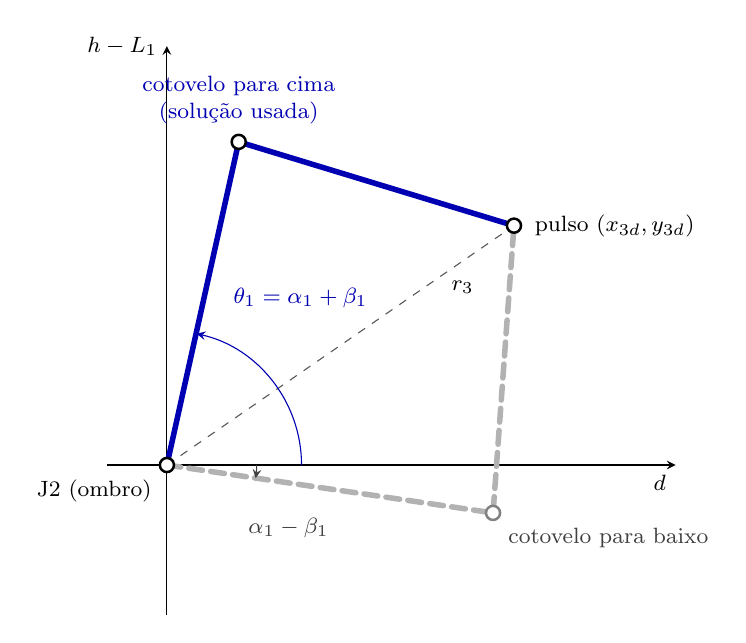
\begin{tikzpicture}[scale=0.38, >=stealth,
    elo/.style={line width=2pt, line cap=round},
    junta/.style={circle, draw, fill=white, line width=0.9pt, inner sep=1.8pt},
    cota/.style={gray!70!black, thin},
    ang/.style={->, thin},
    every node/.style={font=\footnotesize}]

  \draw[->, thin] (-2,0) -- (17,0) node[below left] {$d$};
  \draw[->, thin] (0,-5) -- (0,14) node[left] {$h - L_1$};
  \draw[cota, dashed] (0,0) -- node[pos=0.8, below right=-1pt, black] {$r_3$} (11.6,8.0);
  \draw[elo, gray!60, dash pattern=on 5pt off 3pt] (0,0) -- (10.9,-1.6) -- (11.6,8.0);
  \draw[elo, blue!70!black] (0,0) -- (2.4,10.8) -- (11.6,8.0);
  \node[junta] at (0,0) {}; \node[below left=2pt] at (0,0) {J2 (ombro)};
  \node[junta] at (2.4,10.8) {}; \node[above=3pt, blue!70!black, align=center] at (2.4,10.8) {cotovelo para cima\\(solução usada)};
  \node[junta, draw=gray] at (10.9,-1.6) {}; \node[below right=2pt, gray!50!black, align=center] at (10.9,-1.6) {cotovelo para baixo};
  \node[junta] at (11.6,8.0) {}; \node[right=4pt] at (11.6,8.0) {pulso $(x_{3d}, y_{3d})$};
  \draw[ang, blue!70!black] (4.5,0) arc[start angle=0, end angle=77.2, radius=4.5];
  \node[blue!70!black, anchor=west] at (1.9,5.6) {$\theta_1 = \alpha_1 + \beta_1$};
  \draw[ang, gray!50!black] (3,0) arc[start angle=0, end angle=-8.4, radius=3];
  \node[gray!50!black, anchor=west] at (2.4,-2.1) {$\alpha_1 - \beta_1$};
\end{tikzpicture}
    }
    \caption{Representação das soluções com o cotovelo para cima e para baixo, para uma mesma posição do pulso.}
    \label{fig:cima_baixo}
\end{figure}

Na implementação desenvolvida, é selecionada a solução com o cotovelo orientado para cima, correspondente a $q_3\leq0$.

Esta configuração permite, geralmente, manter o cotovelo numa posição mais elevada, reduzindo o risco de aproximação excessiva à superfície de trabalho e aos objetos presentes no cenário.

\subsection{Junta 4 e passagem para os ângulos das juntas}

Após determinar os ângulos do braço planar, é necessário calcular a rotação da junta J4, de modo a garantir que a garra apresenta a orientação pretendida.

Num manipulador planar de três graus de liberdade, a orientação do último elo resulta da soma dos ângulos articulares.

No myCobot~280, o elo $L_4$ encontra-se perpendicular à direção longitudinal da garra, apresentando uma orientação de $\alpha_3+90^\circ$ relativamente à horizontal.

Deste modo, o ângulo associado à terceira rotação do modelo planar é:

\begin{equation}
    \theta_3=
    (\alpha_3+90^\circ)-\theta_1-\theta_2
    \label{eq:ik_theta3}
\end{equation}

Para converter os ângulos obtidos em valores articulares do manipulador, considera-se a configuração de referência, na qual o primeiro elo apresenta uma orientação de $90^\circ$ relativamente à horizontal quando $q_2=0^\circ$.

Assim, os ângulos das juntas são determinados por:

\begin{equation}
    \boxed{
    \begin{aligned}
        q_2 &= \theta_1-90^\circ\\
        q_3 &= \theta_2\\
        q_4 &= \theta_3\\
        q_5 &= 0^\circ
    \end{aligned}
    }
    \label{eq:ik_q234}
\end{equation}

A junta J5 é mantida a $0^\circ$ na cinemática inversa implementada, permitindo conservar a garra no plano de movimento considerado durante a resolução geométrica.

\subsection{Junta 6}

A junta J6 é utilizada para ajustar a orientação dos dedos da garra relativamente ao objeto a manipular.

Quando o sistema de visão fornece a orientação $\gamma$ de um objeto cúbico em torno do eixo vertical $z$, é possível calcular a rotação necessária para alinhar a garra com as suas faces.

Devido à simetria de um cubo no plano horizontal, existem orientações equivalentes separadas por $90^\circ$. Assim, procura-se selecionar a rotação de menor amplitude que permita realizar a preensão.

A expressão utilizada é:

\begin{equation}
    q_6=
    \operatorname{mod}
    (q_1-\gamma+45^\circ,\;90^\circ)
    -45^\circ
    \label{eq:ik_q6}
\end{equation}

Esta operação permite obter um valor de $q_6$ no intervalo $[-45^\circ,45^\circ[$, evitando rotações desnecessárias da garra.

O ajuste da junta J6 é aplicado quando a garra se encontra numa configuração próxima da vertical, considerando a condição $\psi>45^\circ$.

Caso contrário, é definido $q_6=0^\circ$, mantendo a orientação de referência da junta.

\begin{figure}[H]
  \centering
  % Alinhamento da garra com a peça, vista de cima (esboço): a peça tem simetria de 90 graus, por isso |q6| <= 45 graus
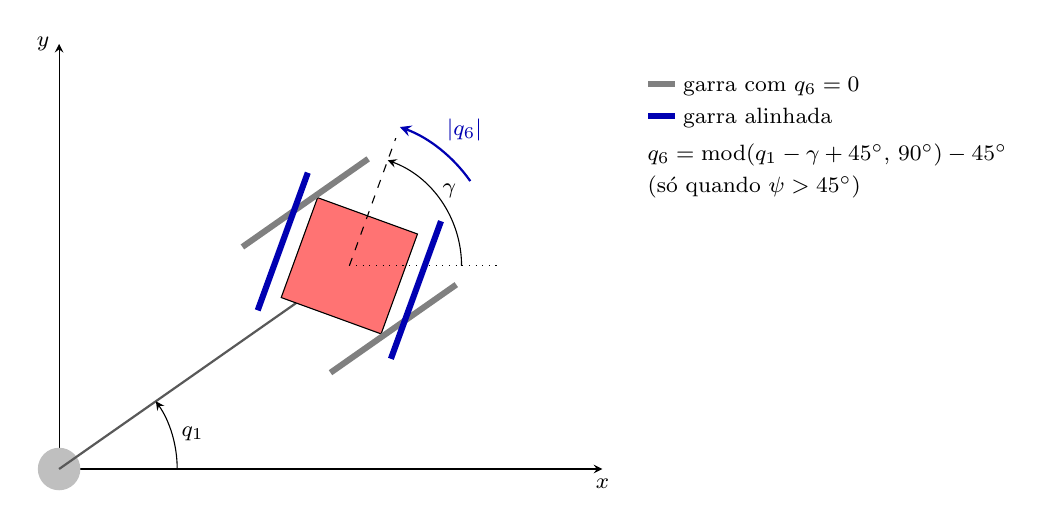
\begin{tikzpicture}[scale=1.5, >=stealth, every node/.style={font=\footnotesize}]
  \def\qa{35}   % direção do braço (q1, esboço)
  \def\ga{70}   % rotação da peça (gamma, esboço)
  % eixos da base
  \draw[->, thin] (0,0) -- (4.6,0) node[below] {$x$};
  \draw[->, thin] (0,0) -- (0,3.6) node[left] {$y$};
  \fill[gray!50] (0,0) circle (0.18);
  % direção do braço
  \draw[gray!70!black, thick] (0,0) -- (\qa:3.0);
  \draw[->, thin] (1.0,0) arc (0:\qa:1.0) node[midway, right] {$q_1$};
  % peça rodada de gamma, centrada no fim do braço
  \begin{scope}[shift={(\qa:3.0)}]
    \begin{scope}[rotate=\ga]
      \fill[red!55] (-0.45,-0.45) rectangle (0.45,0.45);
      \draw (-0.45,-0.45) rectangle (0.45,0.45);
      \draw[thin, dashed] (0,0) -- (1.15,0);
    \end{scope}
    \draw[thin, dotted] (0,0) -- (1.25,0);
    \draw[->, thin] (0.95,0) arc (0:\ga:0.95) node[pos=0.6, right] {$\gamma$};
    % garra na orientação neutra (segue q1)
    \begin{scope}[rotate=\qa]
      \draw[gray, line width=2.2pt] (-0.65,-0.65) -- (0.65,-0.65);
      \draw[gray, line width=2.2pt] (-0.65,0.65) -- (0.65,0.65);
    \end{scope}
    % garra alinhada com a peça
    \begin{scope}[rotate=\ga]
      \draw[blue!70!black, line width=2.2pt] (-0.62,-0.6) -- (0.62,-0.6);
      \draw[blue!70!black, line width=2.2pt] (-0.62,0.6) -- (0.62,0.6);
    \end{scope}
    \draw[->, blue!70!black, thick] (\qa:1.25) arc (\qa:\ga:1.25) node[pos=0.5, above right=-1pt] {$|q_6|$};
  \end{scope}
  % legenda
  \node[align=left, anchor=north west] at (4.9,3.4) {%
    \textcolor{gray}{\rule[0.5ex]{10pt}{2pt}} garra com $q_6 = 0$\\[2pt]
    \textcolor{blue!70!black}{\rule[0.5ex]{10pt}{2pt}} garra alinhada\\[4pt]
    $q_6 = \mathrm{mod}(q_1 - \gamma + 45^\circ,\, 90^\circ) - 45^\circ$\\[2pt]
    (só quando $\psi > 45^\circ$)};
\end{tikzpicture}
  \caption{Alinhamento da garra com a peça, vista de cima (esboço). Como a peça tem simetria de $90^\circ$, a junta J6 roda no máximo $45^\circ$.}
  \label{fig:orientacao_q6}
\end{figure}

\subsection{Soluções rejeitadas}

Embora a abordagem geométrica permita determinar possíveis soluções para a cinemática inversa, nem todas correspondem a configurações válidas do manipulador.

Deste modo, são aplicadas condições adicionais para verificar a viabilidade das soluções obtidas.

Os ângulos articulares são inicialmente normalizados para o intervalo $]-180^\circ,180^\circ]$.

Uma solução é rejeitada quando se verifica alguma das seguintes condições:

\begin{itemize}
    \item \textbf{Limites articulares:}
    algum dos ângulos calculados ultrapassa os limites permitidos para a respetiva junta. Por omissão, são considerados limites de $\pm165^\circ$ para J1 a J5 e de $\pm175^\circ$ para J6. Durante a execução, os limites são obtidos diretamente do modelo do robô;

    \item \textbf{Flexão excessiva do cotovelo:}
    verifica-se $|q_3|>140^\circ$, correspondendo a uma configuração em que o antebraço se aproxima excessivamente do braço. Esta condição é utilizada como restrição adicional para evitar configurações demasiado fechadas;

    \item \textbf{Posicionamento abaixo da base:}
    o cotovelo, a junta J4 ou a junta J5 apresentam uma altura inferior ou igual a zero relativamente ao referencial considerado.
\end{itemize}

As alturas das juntas utilizadas nesta última verificação são determinadas por:

\begin{align}
    z_c &= L_1+L_2\sin\theta_1\\
    z_{J4} &= z_c+
    L_3\sin(\theta_1+\theta_2)\\
    z_{J5} &= z_{J4}+
    L_4\sin\theta_3'
\end{align}

onde:

\begin{equation}
    \theta_3'=\theta_1+\theta_2+\theta_3
\end{equation}

A solução é rejeitada se alguma destas alturas for inferior ou igual a zero.

Adicionalmente, um ponto é considerado geometricamente inalcançável no plano horizontal quando $r<L_5$, não sendo possível determinar um valor real para a distância frontal $d$.

Caso nenhuma das configurações articulares satisfaça as condições estabelecidas, o ponto é considerado inalcançável segundo as restrições e as inclinações testadas pelo algoritmo.

\subsection{Escolha da inclinação}

A orientação da garra constitui um parâmetro importante na resolução da cinemática inversa, uma vez que influencia a posição do pulso e, consequentemente, a possibilidade de alcançar o alvo.

Na implementação desenvolvida, a inclinação preferencial é $\psi=90^\circ$, correspondente à garra orientada verticalmente para baixo.

Quando não é possível encontrar uma solução válida para esta inclinação, o algoritmo procura configurações alternativas, variando progressivamente o ângulo $\psi$ em incrementos de $5^\circ$.

A procura é realizada inicialmente para inclinações superiores a $90^\circ$, aproximando a garra da direção da base, e posteriormente para inclinações inferiores a $90^\circ$, orientando-a para o exterior.

O intervalo de inclinações considerado é:

\begin{equation}
    30^\circ\leq\psi\leq135^\circ
\end{equation}

O limite inferior evita configurações em que a garra se encontra demasiado próxima da horizontal, enquanto o limite superior restringe a inclinação da garra na direção da base.

A Figura~\ref{fig:inclinacao} ilustra as inclinações consideradas e a ordem de procura utilizada pelo algoritmo.

\begin{figure}[H]
    \centering
    \resizebox{0.65\textwidth}{!}{
        % Escolha da inclinação: direção da garra para vários psi à volta do mesmo alvo; unidades em cm
\begin{tikzpicture}[scale=0.38, >=stealth,
    elo/.style={line width=2pt, line cap=round},
    junta/.style={circle, draw, fill=white, line width=0.9pt, inner sep=1.8pt},
    cota/.style={gray!70!black, thin},
    ang/.style={->, thin},
    every node/.style={font=\footnotesize}]

  \draw[->, thin] (-2,0) -- (30,0) node[below left] {$d$};
  \draw[->, thin] (0,-1) -- (0,22) node[left] {$h$};
  \fill[gray!25] (-2.5,-0.8) rectangle (2.5,0); \node[below=8pt] at (0,0) {base};
  \coordinate (T) at (18.9,6.0);
  \fill[blue!8] (T) -- ++(45:15.1) arc[start angle=45, end angle=150, radius=15.1] -- cycle;
  \node[blue!50!black, font=\scriptsize, align=center] at ($(T)+(97:18.3)$) {inclinações permitidas\\$30^\circ \leq \psi \leq 135^\circ$};
  \draw[gray!70, line width=1.2pt, <-] (T) -- ++(150:15.1) node[pos=1.08, font=\scriptsize] {$30^\circ$};
  \draw[gray!70, line width=1.2pt, <-] (T) -- ++(120:15.1) node[pos=1.08, font=\scriptsize] {$60^\circ$};
  \draw[blue!70!black, line width=2pt, <-] (T) -- ++(90:15.1) node[pos=1.08, font=\scriptsize] {$90^\circ$};
  \draw[gray!70, line width=1.2pt, <-] (T) -- ++(60:15.1) node[pos=1.08, font=\scriptsize] {$120^\circ$};
  \draw[gray!70, line width=1.2pt, <-] (T) -- ++(45:15.1) node[pos=1.08, font=\scriptsize] {$135^\circ$};
  \fill (T) circle (6pt); \node[below=3pt] at (T) {alvo};
  \draw[->, thick, orange!85!black] ($(T)+(85:7)$) arc[start angle=85, end angle=50, radius=7];
  \draw[->, thick, violet!80!black] ($(T)+(95:7)$) arc[start angle=95, end angle=145, radius=7];
  \node[align=left, anchor=north west, font=\scriptsize] at (21,9) {1.\ $\psi = 90^\circ$ (garra vertical)\\\textcolor{orange!85!black}{2.\ $\psi > 90^\circ$: para a base}\\\textcolor{violet!80!black}{3.\ $\psi < 90^\circ$: para fora}\\de $5^\circ$ em $5^\circ$, depois bisseção\\[3pt]cada linha: garra (J5 $\to$ alvo)};
\end{tikzpicture}
    }
    \caption{Inclinações da garra consideradas na procura de uma solução válida para a cinemática inversa.}
    \label{fig:inclinacao}
\end{figure}

Quando é encontrada uma inclinação válida, o algoritmo realiza um refinamento através do método da bisseção, procurando uma orientação mais próxima de $90^\circ$ que continue a satisfazer as condições de alcance.

Este procedimento permite obter uma transição mais suave da orientação da garra à medida que o alvo se desloca, evitando alterações bruscas associadas aos incrementos iniciais de $5^\circ$.

Nos movimentos verticais, é mantida uma única inclinação durante toda a trajetória, de forma a preservar a configuração selecionada e reduzir o risco de variações abruptas dos ângulos articulares.

\clearpage
